\chapter{Track A: zero-shot classification}
\label{ch:trackA}

Track~A asks the first half of the research question: \emph{without any training, can a small open VLM tell decline, stable and increase apart from the before/after images and the evidence?} It was run twice: first with the full evidence card (Phase~A, 25--26 September), then without the card's summary line and with equal inputs (Phase~E, 19--20 October). The second run changes how the first must be read.

\section{What was run}

\begin{wherecode}
\textbf{Full card (Phase~A).} Notebooks \file{05_vlm_llava15.ipynb}--\file{08_vlm_blip2.ipynb}, calling \texttt{collate} and \texttt{eval\_combo} in \file{src/vlm_eval.py}. Results: \file{results/vlm_combo_*.json} and \file{results/vlm_combo_comparison.json}.\\
\textbf{Leak-free reruns (Phase~E).} \file{scripts/run_protocol_fair_eval.py} (phases \texttt{qwen-leakfree} and \texttt{fair-four}) on the laptop. Results: \file{results/protocol/}. Commands: \file{docs/PROTOCOL_RERUN.md}.
\end{wherecode}

\begin{itemize}
  \item The same 55 test patches, in the same order, for every run; greedy decoding; one run per model; the small laptop checkpoints of Table~\ref{tab:models}.
  \item \textbf{Full card} (``Condition~C''): Qwen and LLaVA received both images and the full card; PaliGemma both images and one NDVI line; BLIP-2 one stitched image and a short prompt (Table~\ref{tab:inputs}). Run times for 55 patches: LLaVA 403\,s, Qwen 818\,s, BLIP-2 1,879\,s, PaliGemma 3,226\,s.
  \item \textbf{\texttt{evidence\_only}}: the full card with the summary line and label words removed (Qwen only).
  \item \textbf{\texttt{compact}}: the same label-free numeric table for all four models (Chapter~\ref{ch:models}).
\end{itemize}

\section{Results with the full card}

\begin{table}[H]
\centering
\caption{Track~A with the full card, on the 55 test patches (\file{results/vlm_combo_*.json}).}
\label{tab:trackA}
\small
\begin{tabularx}{\textwidth}{L{2.9cm}L{2.5cm}rcrY}
\toprule
Model & Input & Acc. & 95\,\% CI & Macro-F1 & What it answered \\
\midrule
Qwen2-VL-2B & images + full card & 56.4\,\% & 43.3--68.6 & 0.466 & 23 decline, 32 stable, never increase \\
PaliGemma-3B & images + NDVI line & 36.4\,\% & 24.9--49.6 & 0.271 & 42 decline, 13 increase, never stable \\
LLaVA-Interleave-0.5B & images + full card & 32.7\,\% & 21.8--45.9 & 0.164 & ``decrease'' for all 55 \\
BLIP-2 OPT-2.7B & stitched image only & 32.7\,\% & 21.8--45.9 & 0.164 & repeated its prompt (read as decline) \\
\midrule
Always ``increase'' & --- & 34.5\,\% & 23.4--47.7 & 0.171 & baseline \\
\bottomrule
\end{tabularx}
\end{table}

Read on its own, this table says: Qwen2-VL-2B is the only model above the baseline, though not significantly ($p = 0.12$, Table~\ref{tab:mcnemar}); it was right on all 18 decline patches and 13 of 18 stable patches but never answered ``increase''. LLaVA received the same input and answered ``decrease'' every time. PaliGemma and BLIP-2 received far less, and BLIP-2's score is a parsing artefact (Chapter~\ref{ch:models}).

\section{The summary line, and what happens without it}
\label{sec:summaryline}

\subsection{What the line contains}

Every full card ends with the pipeline's summary line (Chapter~\ref{ch:stage03}), for example:

\begin{center}
\small\texttt{Inference for p00575: vegetation\_trend=strong\_decline, burn/deforestation cue=low, candidate\_class=decline}
\end{center}

It carries two things: the card's \textbf{trend word} (\texttt{strong\_decline}, \texttt{moderate\_decline}, \texttt{stable}, \texttt{slight\_greening}, \texttt{greening}) and the \textbf{gold label}. Checked on all 55 test cards, the trend words appear \emph{nowhere else} on the card.

\begin{newinfo}
\textbf{A correction of version~2.} Version~2 of this guide noticed that Qwen's answers agree with the card's trend words on 45 of 55 patches, and that Qwen answered ``stable'' on all 19 increase patches although the line said \texttt{candidate\_class=increase}. It concluded that Qwen ``did not copy the label'' and that this supported a positive reading of 56.4\,\%. The first half is true: Qwen did not copy the label token. The second half was wrong, because the trend words it followed sit in the same line. Qwen depended on the summary line, and the leak-free reruns below confirm it.
\end{newinfo}

\subsection{Results without the line}

\begin{table}[H]
\centering
\caption{Leak-free reruns on the same 55 test patches (\file{results/protocol/}, 19--20 October). Recomputed from the prediction files.}
\label{tab:leakfree}
\small
\begin{tabularx}{\textwidth}{L{2.9cm}L{2.8cm}rcY}
\toprule
Model & Input & Acc. & 95\,\% CI & What it answered \\
\midrule
Qwen2-VL-2B & \texttt{evidence\_only} card & 32.7\,\% (18/55) & 21.8--45.9 & per-patch answers overwritten (see Chapter~\ref{ch:results}) \\
Qwen2-VL-2B & \texttt{compact} table & 32.7\,\% (18/55) & 21.8--45.9 & ``stable'' for all 55 \\
LLaVA-Interleave-0.5B & \texttt{compact} table & 43.6\,\% (24/55) & 31.4--56.7 & 43 decline, 12 increase, never stable; right on 16/18 decline and 8/19 increase \\
PaliGemma-3B & \texttt{compact} table & --- & --- & not loaded (gated model, HTTP 401) \\
BLIP-2 OPT-2.7B & \texttt{compact} table & --- & --- & 0 of 55 answers parsable after the echo fix \\
\bottomrule
\end{tabularx}
\end{table}

\begin{figure}[H]
\centering
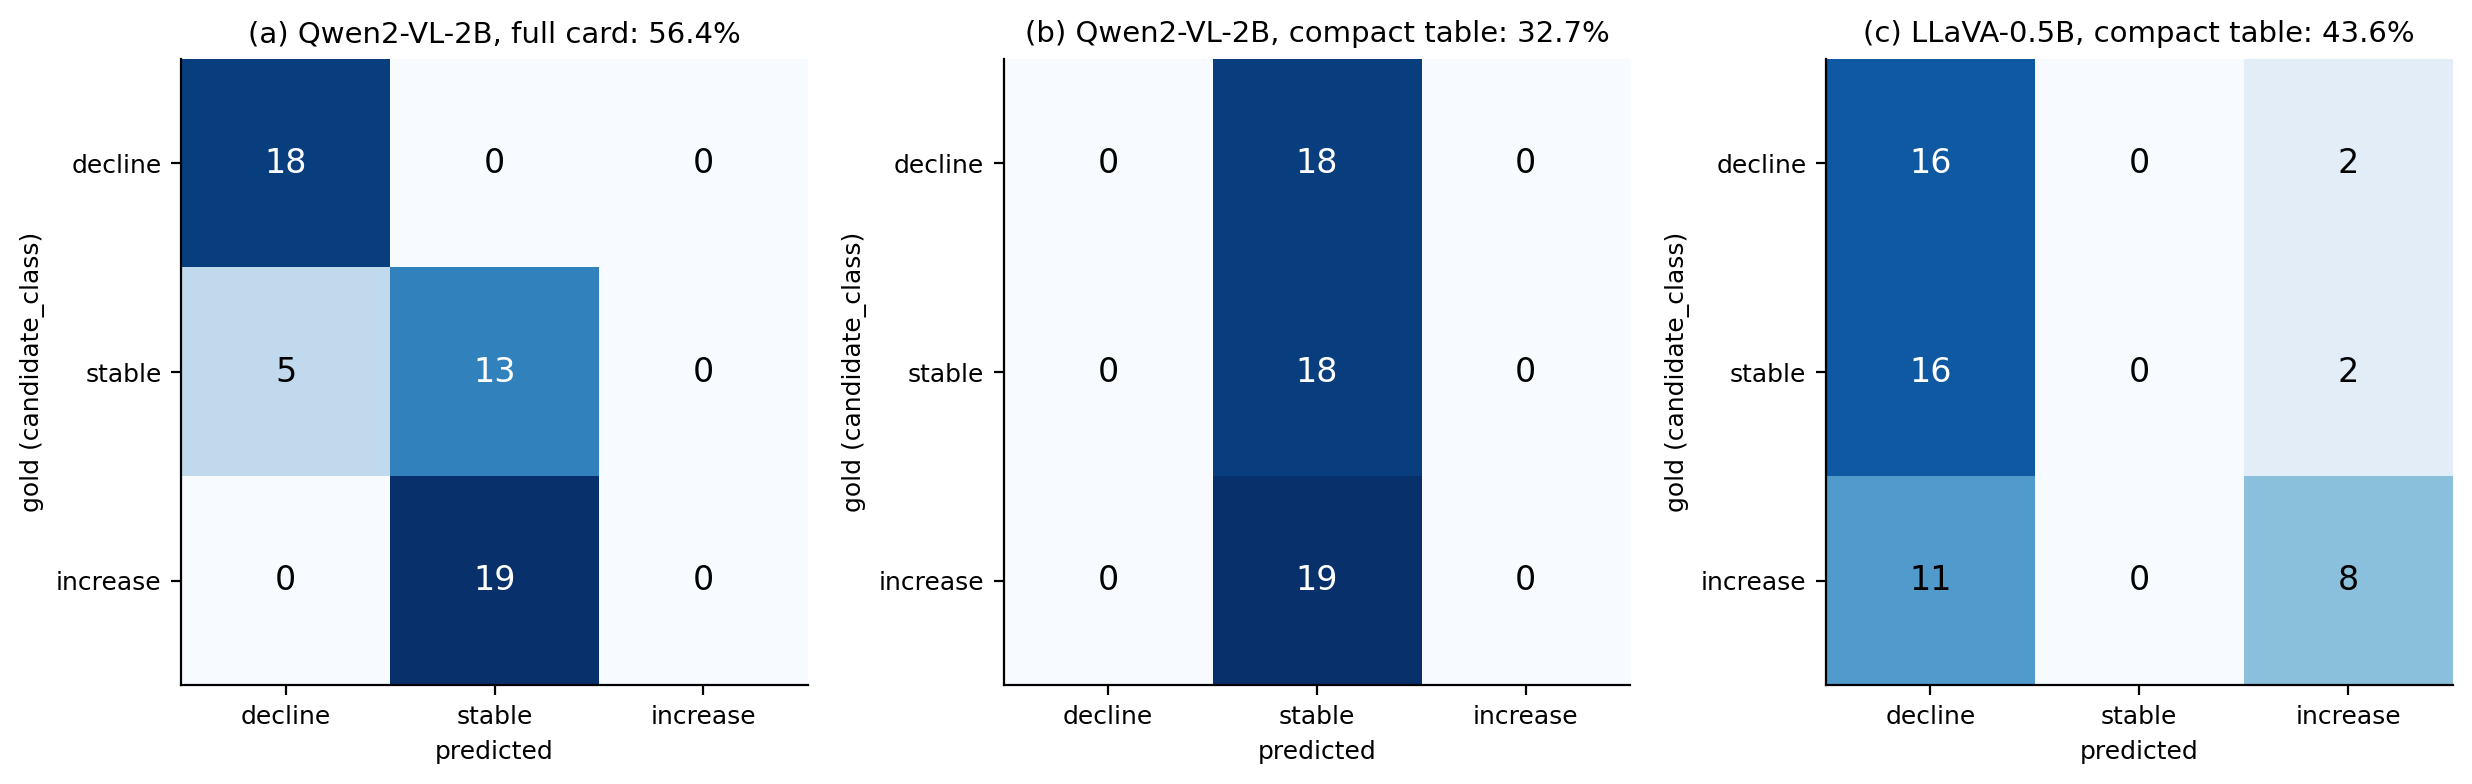
\includegraphics[width=\textwidth]{figures/fig_leakfree_confusion.png}
\caption{Confusion matrices (rows: gold; columns: predicted). (a) Qwen with the full card. (b) Qwen with the label-free compact table: ``stable'' for everything. (c) LLaVA with the compact table. Made by \file{study_guide_v3/make_figures_v3.py}.}
\label{fig:leakfreecm}
\end{figure}

\subsection{How to read them}

\begin{itemize}
  \item \textbf{Qwen's 56.4\,\% came from the summary line.} Without it Qwen falls to 32.7\,\%, the share of stable patches, because it answers ``stable'' for everything. On the patches where the two Qwen runs disagree, the full card wins 18 to 5 ($p = 0.011$): the only significant difference in Track~A.
  \item \textbf{LLaVA does better with a clean table than with the full card} (43.6\,\% against 32.7\,\%; 8 patches gained, 2 lost, $p = 0.11$), and its answers now follow the evidence somewhat: it catches most declines and some increases. But 43.6\,\% is not significantly above the 34.5\,\% baseline ($p = 0.44$), and it never answers ``stable''.
  \item \textbf{No model classifies from the evidence alone} better than guessing. This is now the central classification finding.
  \item The \texttt{compact} table and the \texttt{evidence\_only} card are different inputs (numbers only, versus the descriptive card without its last line), and Qwen scored 32.7\,\% on both.
\end{itemize}

\begin{plainwords}
With the full card, Qwen looked like the one model that could do the task. Without the card's last line it answers ``stable'' to everything. What looked like skill was the model reading a word the pipeline had already written for it. Finding this out, and saying so, is a real result of your project.
\end{plainwords}

\section{The card contains enough information}

A rule that reads one number from the card, the \dndvi{} value, and compares it with two cut-offs fitted on the training split ($-0.032$ and $-0.0011$; 96.1\,\% training accuracy) gets \textbf{52 of 55} test patches right (\textbf{94.5\,\%}, interval 85.1--98.1\,\%). With the fixed $\pm0.02$ cut-offs it gets 63.6\,\%. The rule is not a forest-change detector, since it reproduces how the labels were made, but it shows that every model in Table~\ref{tab:leakfree} had the answer in front of it as a number and did not use it.

\begin{watchout}
Another pair of cut-offs ties with this one on the training data and scores 96.4\,\% on test. Report 94.5\,\% with its cut-offs, and say how they were chosen (the first pair with the highest training accuracy).
\end{watchout}

\section{Earlier supporting analyses}

\begin{figure}[H]
\centering
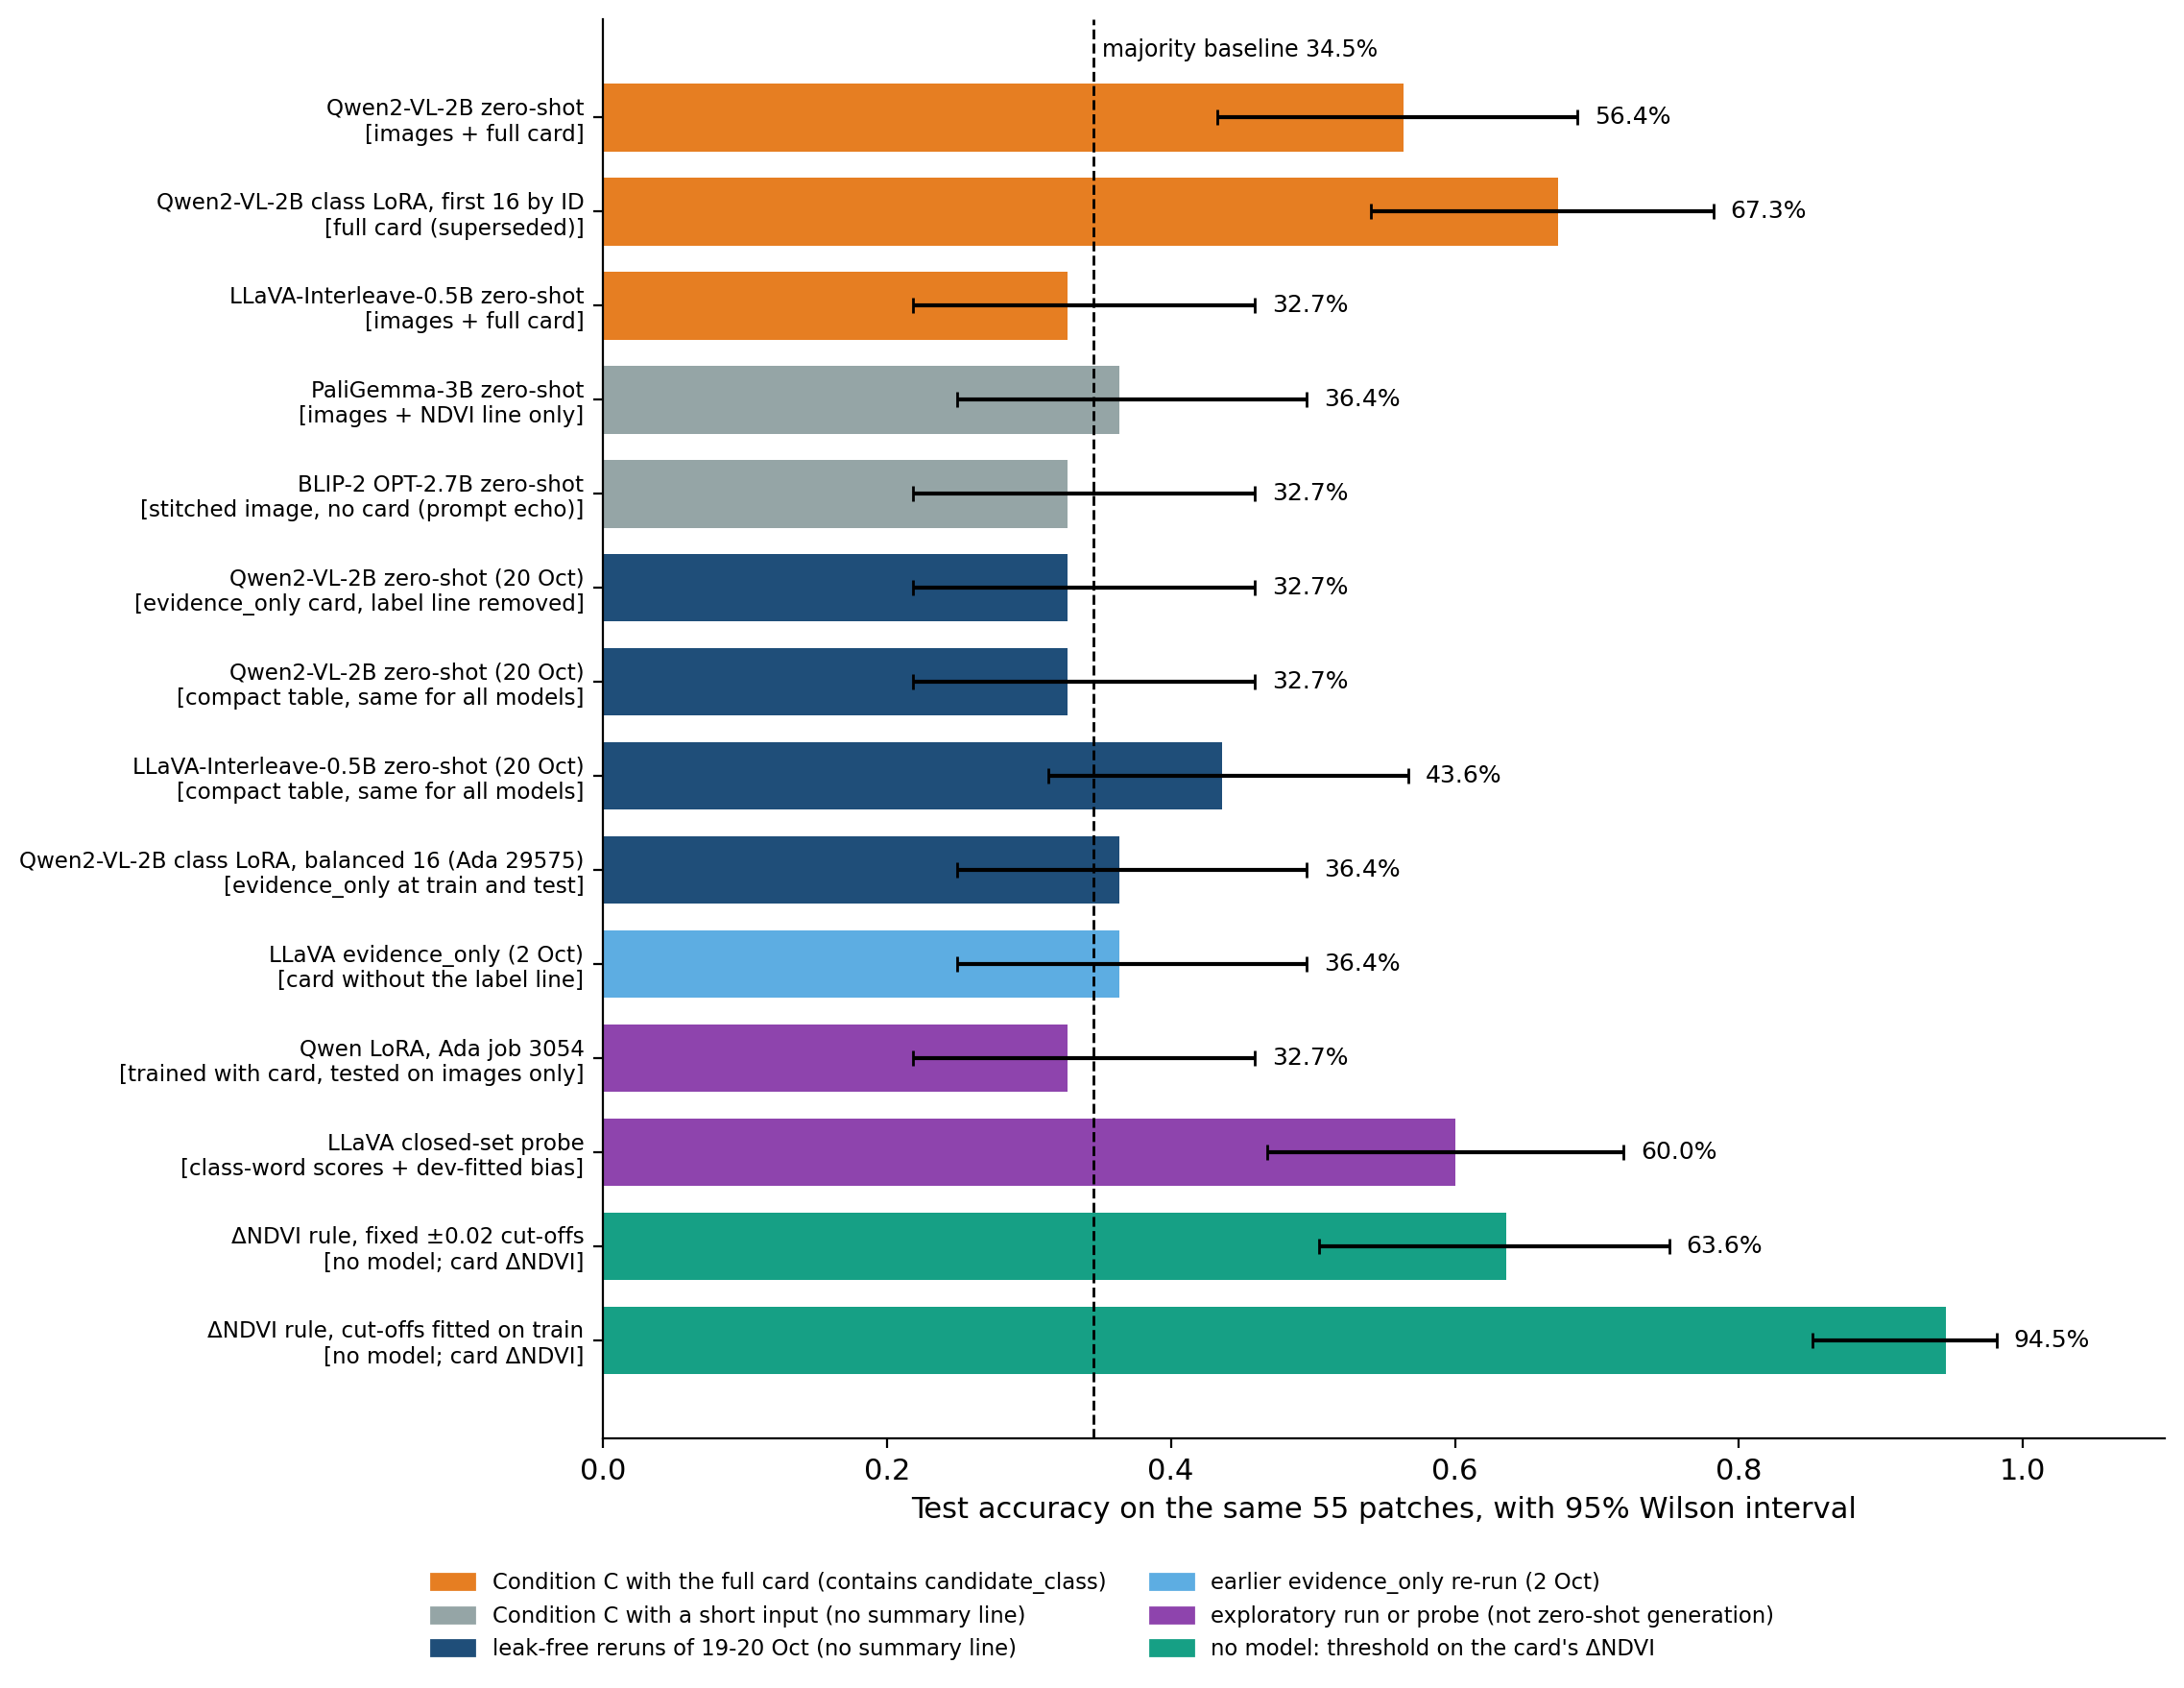
\includegraphics[width=\textwidth]{figures/fig_accuracy_v3.png}
\caption{Every classification run on the same 55 test patches, labelled by what the model was given, with 95\,\% Wilson intervals. Dark blue: the leak-free reruns of 19--20 October. Made by \file{study_guide_v3/make_figures_v3.py}.}
\label{fig:accv2}
\end{figure}

\paragraph{The 2 October \texttt{evidence\_only} re-run.} LLaVA 36.4\,\%, PaliGemma 36.4\,\% and BLIP-2 32.7\,\% (\file{results/explain/oneword_*.json}). Only LLaVA's input changed; PaliGemma and BLIP-2 never had the line. This run is now superseded by the Phase~E reruns, which also cover Qwen.

\paragraph{The closed-set probe.} \file{src/vlm_closedset.py} (Ada, 2 October) scores each class word's likelihood with a four-panel image, a prompt stating the $\pm0.02$ rule, and three biases fitted on the development set. LLaVA reached 60.0\,\% (33/55) but never answered ``stable'' and matched the stated rule on only 25 patches; PaliGemma and BLIP-2 answered ``stable'' for everything (32.7\,\%). It is a probe with a tuned bias, not a zero-shot result.

\paragraph{The exploratory Ada fine-tune tested on images only} (job 3054, 32.7\,\%) belongs to Track~B (Chapter~\ref{ch:trackB}).

\begin{figure}[H]
\centering
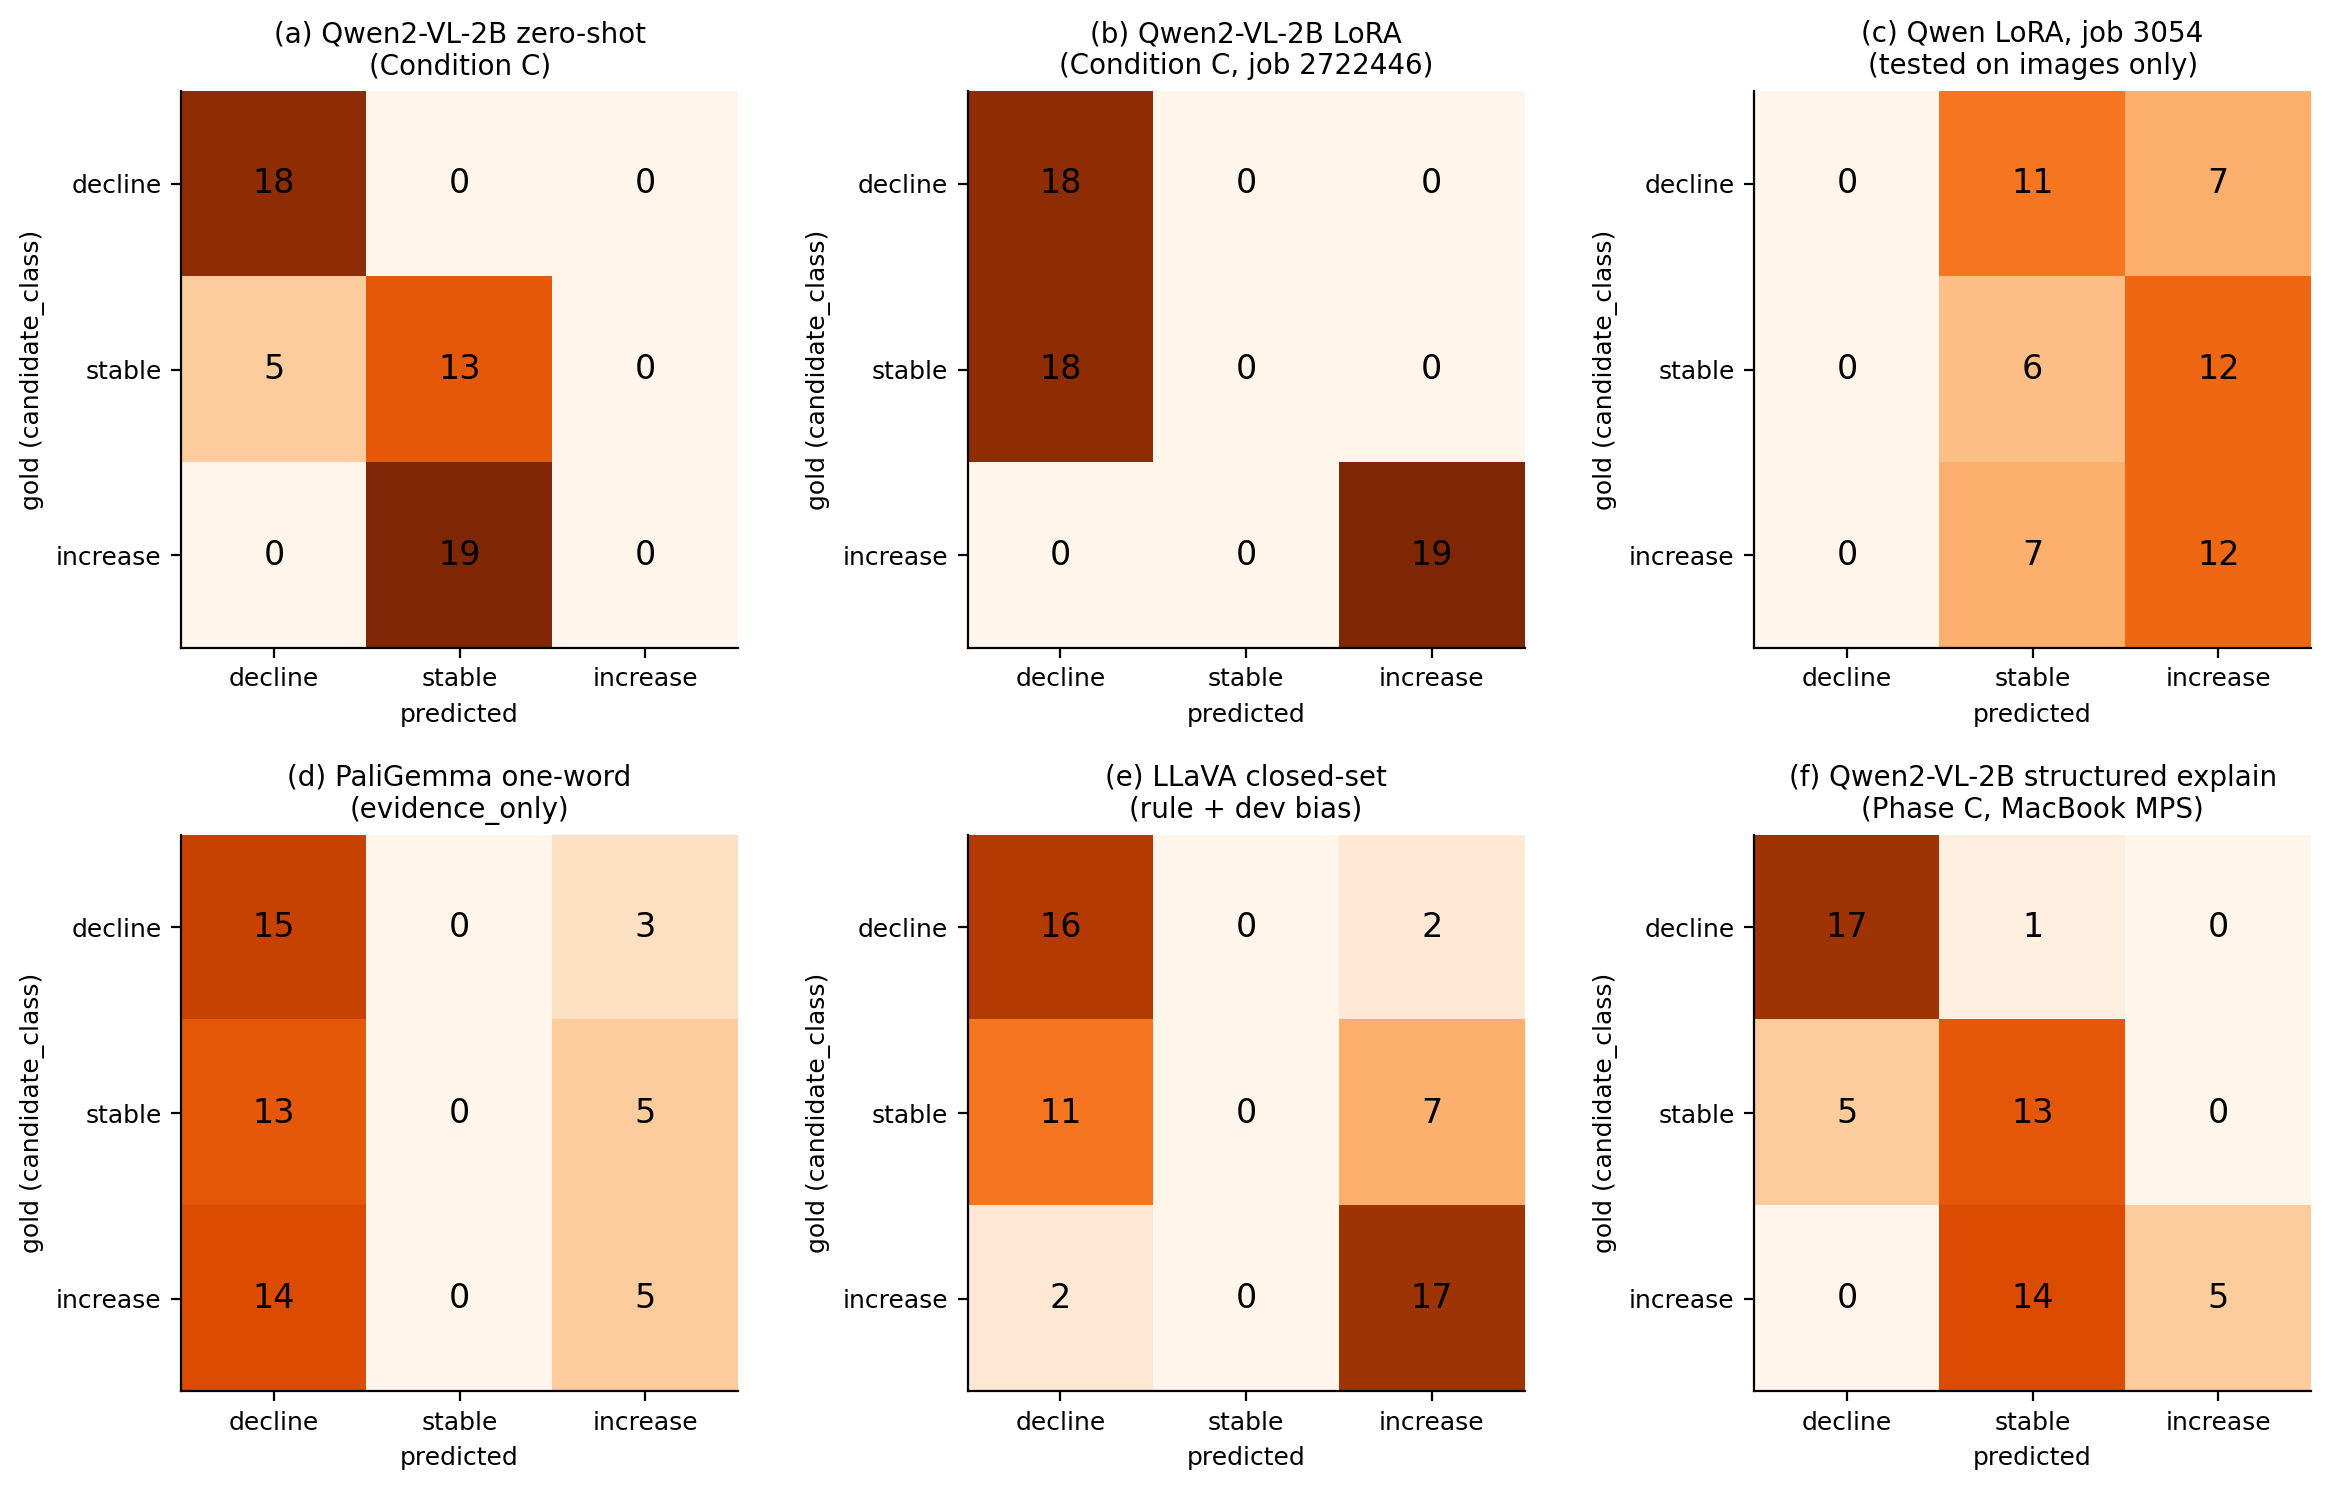
\includegraphics[width=\textwidth]{figures/fig_confusion.png}
\caption{Confusion matrices from the first two phases. (a) Qwen zero-shot and (b) the old Qwen class LoRA, both with the full card; (c) an exploratory fine-tune tested on images only; (d) PaliGemma with the summary line removed (its input was in fact unchanged); (e) the closed-set LLaVA probe; (f) Qwen with the structured explanation prompt.}
\label{fig:confusionA}
\end{figure}

\section{How this compares with other work}

\begin{itemize}
  \item Established forest-change methods work directly on spectral numbers and time series: global forest-loss maps \citep{hansen2013}, LandTrendr \citep{kennedy2010}, CCDC \citep{zhu2014}, radar alerts \citep{reiche2021}, and change-detection networks trained on image pairs \citep{daudt2018}. The threshold baseline is a minimal version of that approach, and it wins easily.
  \item Remote-sensing VLMs and datasets, such as GeoChat \citep{kuckreja2024}, remote-sensing question answering \citep{lobry2020} and change captioning \citep{liu2022levircc}, depend on large remote-sensing training sets. The models here were trained mainly on everyday photographs, and the forest chips are dark and nearly identical between years (Figure~\ref{fig:examples}).
\end{itemize}

\begin{figure}[H]
\centering
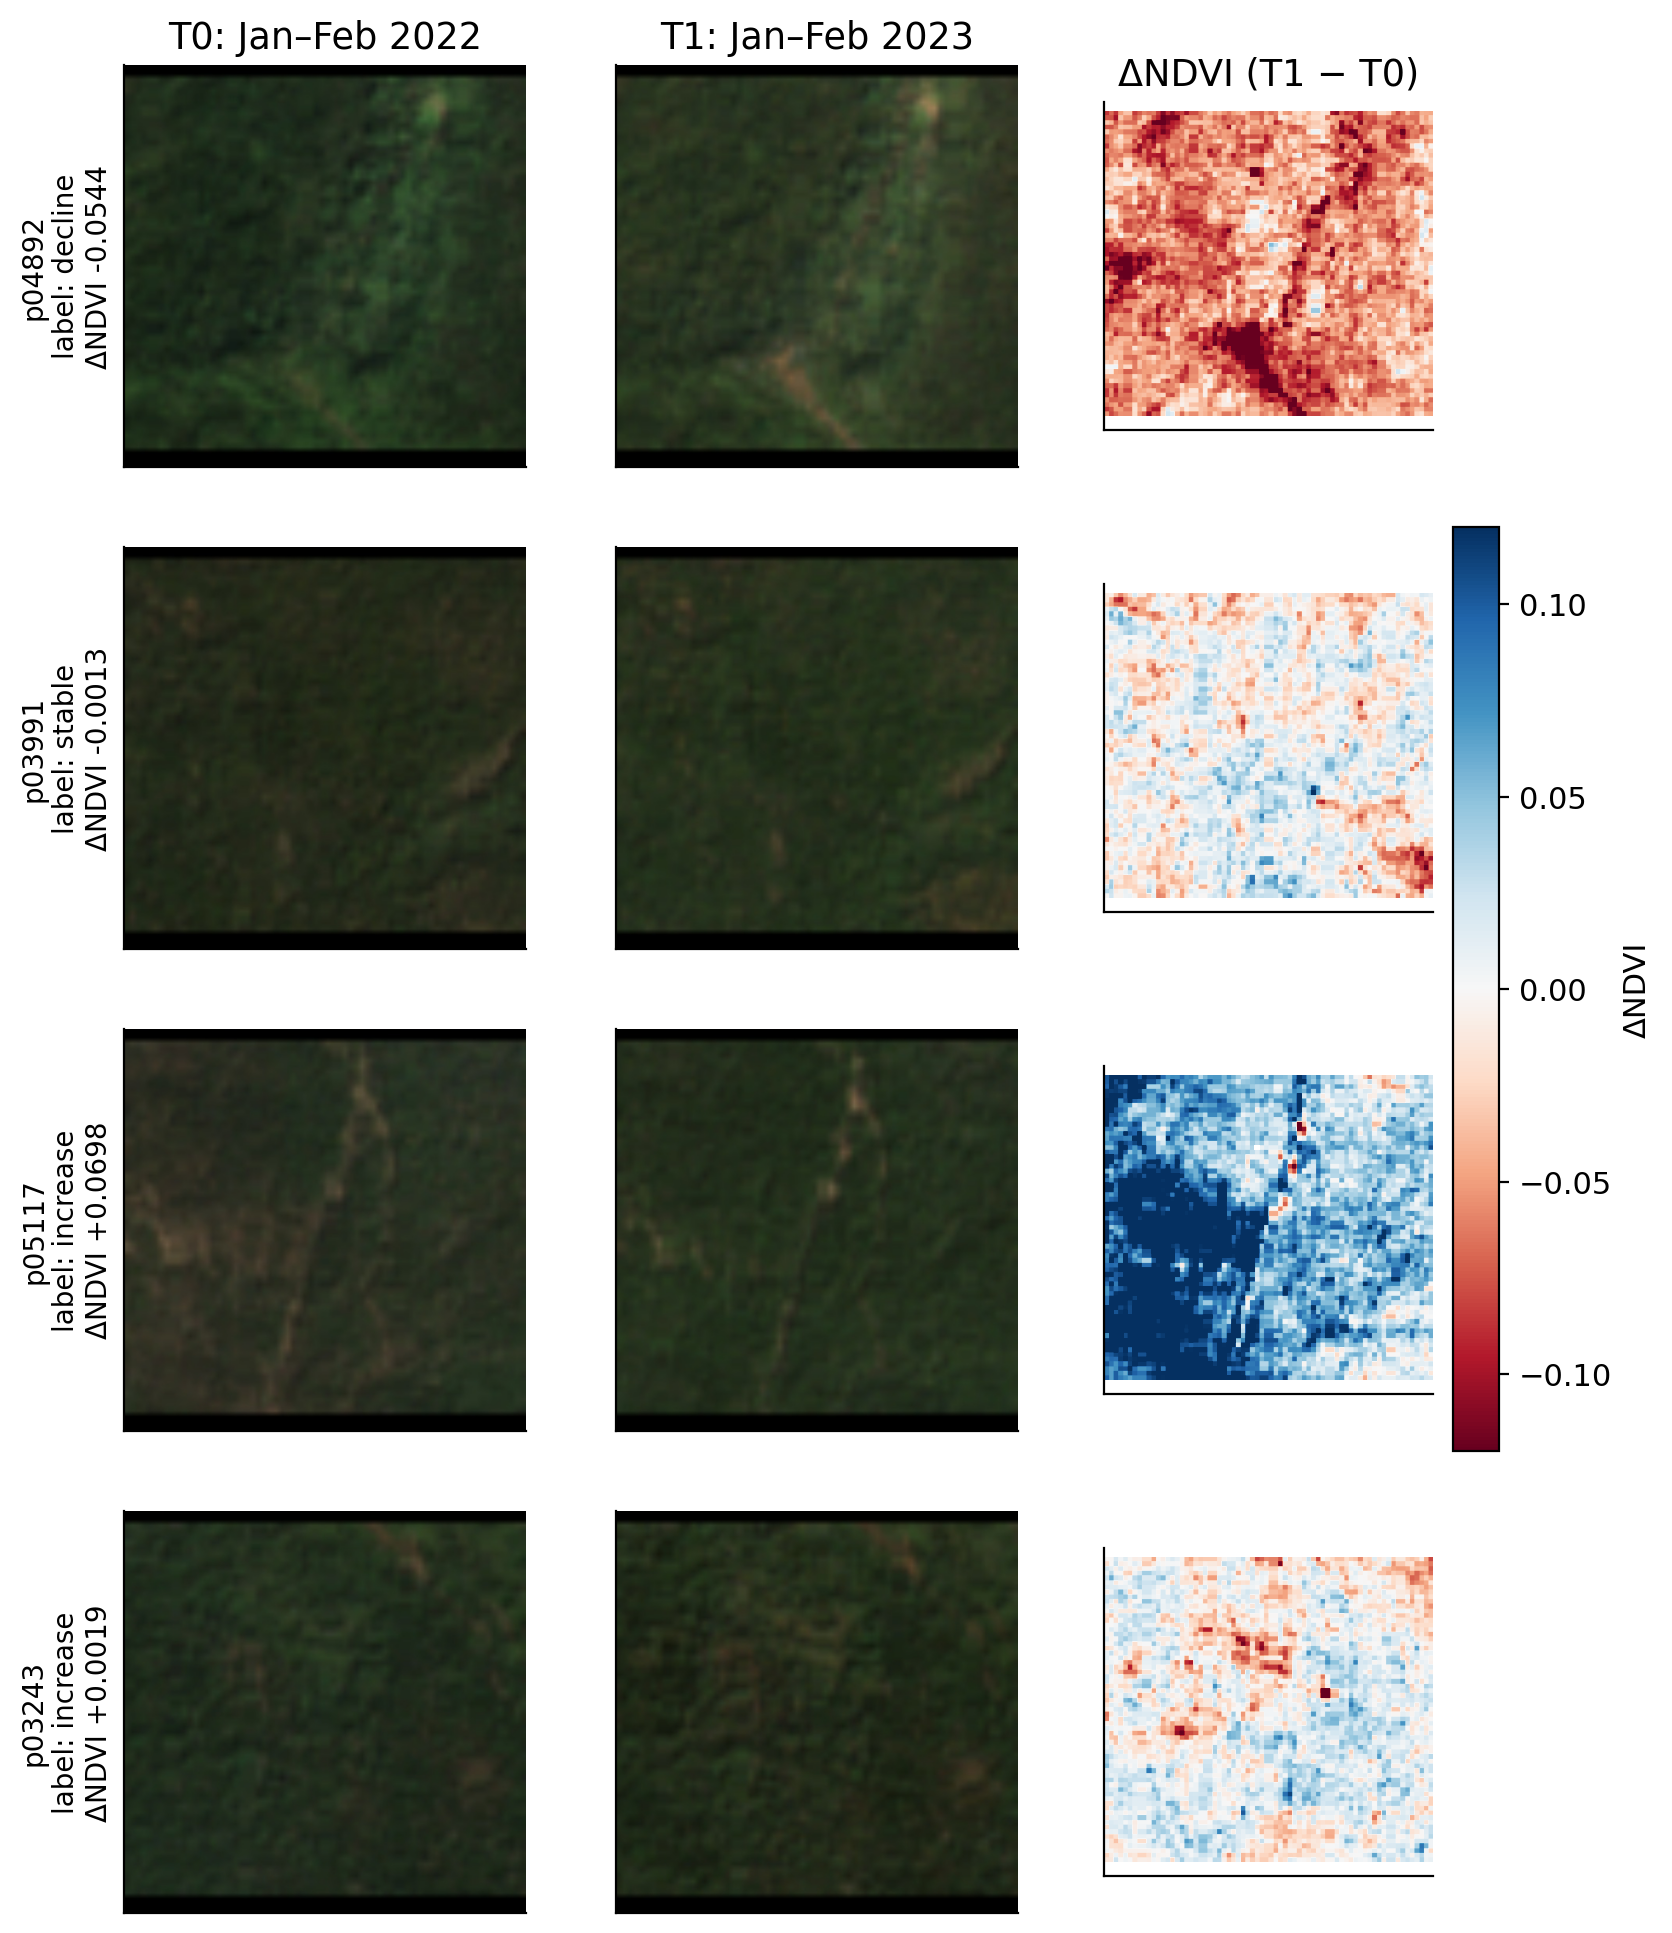
\includegraphics[width=0.78\textwidth]{figures/fig_examples.png}
\caption{Four test patches: the largest NDVI drop among test decline patches (p04892), a typical stable patch (p03991), the largest gain among test increase patches (p05117), and the smallest gain labelled increase (p03243). The \dndvi{} maps show the change clearly; the colour pairs mostly do not. Black bands are padding.}
\label{fig:examples}
\end{figure}

\begin{foryourreport}
In ``Zero-Shot Model Performance'' (about 700 words):
\begin{itemize}
  \item One table in two blocks (Chapter~\ref{ch:results}): the leak-free runs first (Table~\ref{tab:leakfree}), then the full-card runs (Table~\ref{tab:trackA}), each with an \emph{Input} column, intervals and the baselines.
  \item The summary line: what it contains (trend word and label) and what removing it does to Qwen (56.4\,\% $\rightarrow$ 32.7\,\%, $p = 0.011$). Figure~\ref{fig:leakfreecm} shows it at a glance.
  \item LLaVA's 43.6\,\% with the equal-input table, and why it is not significant.
  \item Why PaliGemma and BLIP-2 have no leak-free score (gated model; no parsable answers), and that BLIP-2's earlier 32.7\,\% was an echo.
  \item The 94.5\,\% threshold baseline: the information was on the card.
  \item Do \emph{not} write that Qwen ``did not copy the label'' as evidence for its skill (Section~\ref{sec:summaryline}).
\end{itemize}
\end{foryourreport}

\begin{selfcheck}
\begin{enumerate}
  \item What two pieces of information does the summary line carry?
  \item Why was version~2's claim that Qwen's 56.4\,\% ``did not come from copying'' misleading?
  \item What did Qwen answer once the summary line was removed, and what accuracy does that give?
  \item Is LLaVA's 43.6\,\% evidence that it can classify? Give two reasons for your answer.
  \item Why do PaliGemma and BLIP-2 have no leak-free result?
  \item What does the 94.5\,\% threshold rule show about the models?
\end{enumerate}
\end{selfcheck}
